\documentclass[11pt,a4paper]{article}
\usepackage[T1]{fontenc}
\usepackage{lmodern}
\usepackage{microtype}
\usepackage[margin=2.6cm]{geometry}
\usepackage{amsmath,amssymb,amsthm}
\usepackage{booktabs}
\usepackage{tikz}
\usepackage{pgfplots}
\pgfplotsset{compat=1.18}
\usepackage[hidelinks]{hyperref}
\usepackage{caption}

\newtheorem{proposition}{Proposition}

\definecolor{blue}{HTML}{2E6FBA}
\definecolor{red}{HTML}{C0392B}
\definecolor{stoneb}{HTML}{DCE8F6}
\definecolor{stoner}{HTML}{F6DCD9}

% \stone{x}{y}{top}{right}{bottom}{left}{colour}{fill}
\newcommand{\spikes}[3]{% #1 count, #2 colour, rotation applied outside
  \ifcase#1\or
    \fill[#2] (-0.09,0.5) -- (0,0.66) -- (0.09,0.5) -- cycle;\or
    \fill[#2] (-0.24,0.5) -- (-0.15,0.66) -- (-0.06,0.5) -- cycle; \fill[#2] (0.06,0.5) -- (0.15,0.66) -- (0.24,0.5) -- cycle;\or
    \fill[#2] (-0.33,0.5) -- (-0.24,0.66) -- (-0.15,0.5) -- cycle; \fill[#2] (-0.09,0.5) -- (0,0.66) -- (0.09,0.5) -- cycle; \fill[#2] (0.15,0.5) -- (0.24,0.66) -- (0.33,0.5) -- cycle;\fi}
\newcommand{\stone}[8]{\begin{scope}[shift={(#1,#2)}, scale=0.74]
  \filldraw[fill=#8, draw=#7, thick, rounded corners=1.5pt] (-0.5,-0.5) rectangle (0.5,0.5);
  \begin{scope}[rotate=0]\spikes{#3}{#7}{}\end{scope}
  \begin{scope}[rotate=-90]\spikes{#4}{#7}{}\end{scope}
  \begin{scope}[rotate=180]\spikes{#5}{#7}{}\end{scope}
  \begin{scope}[rotate=90]\spikes{#6}{#7}{}\end{scope}
\end{scope}}

\title{Chain Stones on the $3\times3$ board is a first-player game}
\author{Louis Vandenbruwaene}
\date{October 2026}

\begin{document}
\maketitle

\begin{abstract}
\noindent
Chain Stones is a two-player placement game in which stones with 0 to 3 spikes per side clash with their neighbours. Both players receive hands of equal total strength from a random deal. We solve the $3\times3$ game exactly for 9{,}000 random deals. Under perfect play the first player wins $64.7\% \pm 1.0\%$ of deals and draws are impossible. Openings in a corner are optimal in $95\%$ of deals, while in a typical won deal $91\%$ of all openings throw the win away. Among hands of equal total strength, the hand with its spikes concentrated on fewer sides wins more often. The $4\times4$ game remains unsolved.
\end{abstract}

\section{The game}

Chain Stones is played on an $n\times n$ board by Blue and Red. A \emph{stone} is a square tile with $0$ to $3$ spikes on each of its four sides. Each player holds a hand of stones (five each on $3\times3$, eight each on $4\times4$). Players alternate, Blue first, placing one stone from their hand on an empty square.

\paragraph{Clash.} When a stone is placed, every side that touches an \emph{enemy} stone fights the facing side of that stone, unless both sides are blank. Facing spikes break off one for one. If the new side has spikes left over, the enemy stone is taken and changes colour. If the enemy side has spikes left over, the new stone is taken by the enemy. Both can happen in one move: the new stone takes every neighbour it beats, and is itself taken if it loses any clash. Broken spikes stay broken, and taken stones keep fighting later with whatever spikes remain. Own stones never fight, and a taken stone does not trigger further clashes (an earlier version had chain reactions, which gave the game its name). Figure~\ref{fig:clash} shows an example.

\paragraph{End.} The game ends when the board is full. Each player scores the stones of their colour on the board, and the higher score wins. On $3\times3$ Blue places five stones and Red four, so one red stone stays in hand.

\paragraph{The deal.} For each of the $k$ stone slots a total $t \in \{3,\dots,8\}$ is drawn uniformly. Both players receive a stone with total $t$ in that slot, but the spikes are distributed independently and at random over the four sides (at most $3$ per side). The two hands therefore have the same total strength and differ only in shape.

\begin{figure}[ht]
\centering
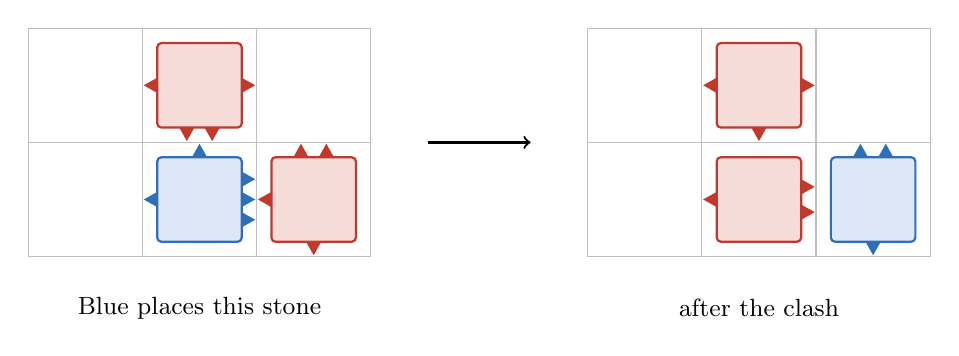
\begin{tikzpicture}[scale=1.45]
  % before
  \draw[gray!50, shift={(-0.5,-0.5)}] (0,0) grid (3,2);
  \stone{2}{0}{2}{0}{1}{1}{red}{stoner}
  \stone{1}{1}{0}{1}{2}{1}{red}{stoner}
  \stone{1}{0}{1}{3}{0}{1}{blue}{stoneb}
  \node[font=\small] at (1,-0.95) {Blue places this stone};
  \draw[->, thick] (3.0,0.5) -- (3.9,0.5);
  % after
  \begin{scope}[xshift=4.9cm]
  \draw[gray!50, shift={(-0.5,-0.5)}] (0,0) grid (3,2);
  \stone{2}{0}{2}{0}{1}{0}{blue}{stoneb}
  \stone{1}{1}{0}{1}{1}{1}{red}{stoner}
  \stone{1}{0}{0}{2}{0}{1}{red}{stoner}
  \node[font=\small] at (1,-0.95) {after the clash};
  \end{scope}
\end{tikzpicture}
\caption{Blue places a stone with spikes $(1,3,0,1)$ (top, right, bottom, left). On the right, $3$ spikes meet $1$: one each breaks and Blue takes the stone. On top, $1$ spike meets $2$: one each breaks and Red wins, so the new stone turns red. Net effect for Blue: one stone gained, one lost.}
\label{fig:clash}
\end{figure}

\section{Method}

\paragraph{Value.} For a deal we define its \emph{value} as the final score of Blue minus that of Red under perfect play by both sides. This is the minimax value of a finite game tree of depth $n^2$.

\paragraph{Solver.} We compute the value with negamax search, alpha-beta pruning and a transposition table keyed by a Zobrist hash of the board (owner and remaining spikes on every square), the stones still in each hand and the side to move. Moves are ordered by their immediate gain, and identical stones in one hand are searched only once. A $3\times3$ deal needs a median of $1.0\times10^{6}$ nodes and about $0.06$ seconds on one core of an Apple M5.

\paragraph{Verification.} The solver re-implements the rules in C. To check it against the game itself, we played 20{,}000 random games ($10{,}000$ on each board size) with the JavaScript rules engine from the game's source and replayed every move in the C engine. All final positions, owners and remaining spikes agree. As a check of the check, removing one rule from the C engine (the new stone being taken after a lost clash) produces 19{,}372 mismatches.

\paragraph{Sample.} We solved 9{,}000 deals drawn with the game's own deal procedure and a seeded random generator. For 500 further deals we also solved every one of the $45$ possible openings (stone, square) separately.

\section{Results}

\begin{proposition}\label{prop:nodraw}
On the $3\times3$ board every game ends with an odd score difference, so draws are impossible.
\end{proposition}
\begin{proof}
A placed stone is never removed, it can only change colour. At the end all $9$ squares hold a stone of one of the two colours, so the scores satisfy $b + r = 9$ and $b - r = 9 - 2r$ is odd.
\end{proof}

\paragraph{First-player advantage.} Table~\ref{tab:values} gives the distribution of values. Blue wins $5{,}826$ of the $9{,}000$ deals, a share of $64.7\%$ with a $95\%$ confidence interval of $63.7\%$ to $65.7\%$. Almost all games are decided by a single stone. In an earlier test, the game's strongest computer player (a time-limited alpha-beta search) won $50$ of $90$ games as Blue against itself.

\begin{table}[ht]
\centering
\begin{tabular}{lrrrrr}
\toprule
value (Blue $-$ Red) & $-3$ & $-1$ & $+1$ & $+3$ & $+5$ \\
\midrule
deals & 26 & 3{,}148 & 5{,}407 & 414 & 5 \\
share & 0.3\% & 35.0\% & 60.1\% & 4.6\% & 0.1\% \\
\bottomrule
\end{tabular}
\caption{Exact values of 9{,}000 random $3\times3$ deals. The mean value is $+0.38$ stones in favour of Blue.}
\label{tab:values}
\end{table}

\paragraph{Openings.} Over 500 deals with all $45$ openings solved:
\begin{itemize}
  \item some corner opening is optimal in $95.2\%$ of deals, some edge opening in $74.0\%$, and the centre in $51.0\%$. Per square, each corner is optimal in $60\%$ to $62\%$ of deals, each edge and the centre in $51\%$ to $54\%$ (figure~\ref{fig:board}).
  \item The game is sharp. In the $321$ deals that Blue wins, on average $87\%$ of the $45$ openings lose (median $91\%$), and no won deal is won by every opening.
  \item Playing the weakest stone first is optimal in $74\%$ of deals, the strongest in $55\%$.
\end{itemize}

\begin{figure}[ht]
\centering
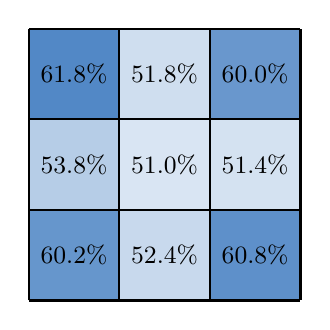
\begin{tikzpicture}[scale=1.15]
  \foreach \v [count=\i from 0] in {61.8,51.8,60.0,53.8,51.0,51.4,60.2,52.4,60.8}{
    \pgfmathtruncatemacro{\x}{mod(\i,3)}
    \pgfmathtruncatemacro{\y}{2-floor(\i/3)}
    \pgfmathsetmacro{\shade}{(\v-48)*6}
    \fill[blue!\shade!white] (\x,\y) rectangle ++(1,1);
    \node at (\x+0.5,\y+0.5) {\small $\v\%$};
  }
  \draw[thick] (0,0) grid (3,3);
\end{tikzpicture}
\caption{Share of 500 deals in which a first stone on this square is optimal for Blue (for the best choice of stone). Corners are the strongest opening squares.}
\label{fig:board}
\end{figure}

\paragraph{What makes a hand strong.} Both hands have the same total number of spikes, so they differ only in how the spikes are spread. Let $z$ be the number of blank sides in a hand. Figure~\ref{fig:zero} shows Blue's winning share against $z_{\text{Blue}} - z_{\text{Red}}$. The share rises from $30\%$ to $93\%$ as Blue's hand gets more blank sides than Red's. More blank sides at the same total means more spikes on the remaining sides, and a side with $3$ spikes never loses a clash. The difference in the number of $3$-spike sides shows the same trend (from $33\%$ to $98\%$).

\begin{figure}[ht]
\centering
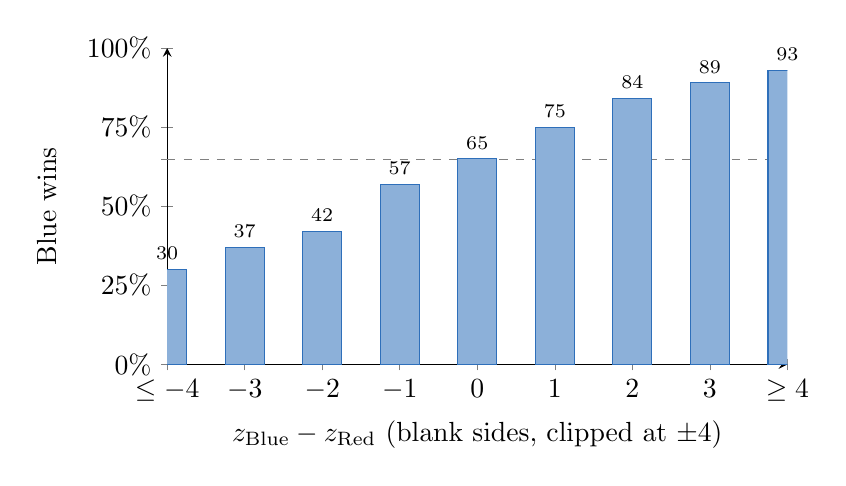
\begin{tikzpicture}
\begin{axis}[
  width=0.78\textwidth, height=5.6cm,
  ybar, bar width=14pt, enlarge x limits=0.08,
  ymin=0, ymax=1,
  xlabel={$z_{\text{Blue}} - z_{\text{Red}}$ (blank sides, clipped at $\pm4$)},
  ylabel={Blue wins},
  xtick={-4,...,4},
  xticklabels={$\le -4$,$-3$,$-2$,$-1$,$0$,$1$,$2$,$3$,$\ge 4$},
  ytick={0,0.25,0.5,0.75,1},
  yticklabels={0\%,25\%,50\%,75\%,100\%},
  axis lines=left,
  nodes near coords={\pgfmathprintnumber[fixed,precision=0]{\pgfplotspointmeta}},
  point meta={y*100},
  every node near coord/.append style={font=\scriptsize},
  extra y ticks={0.647}, extra y tick labels={}, extra y tick style={grid=major, grid style={dashed, gray}},
]
\addplot[fill=blue!55, draw=blue] coordinates {(-4,0.30) (-3,0.37) (-2,0.42) (-1,0.57) (0,0.65) (1,0.75) (2,0.84) (3,0.89) (4,0.93)};
\end{axis}
\end{tikzpicture}
\caption{Blue's winning share against the difference in blank sides between the two hands, over 9{,}000 deals. The dashed line is the overall share of $64.7\%$.}
\label{fig:zero}
\end{figure}

\section{The $4\times4$ board}

On $4\times4$ each player places all eight stones. The full game tree has up to $\prod_{j=0}^{7}(8-j)^2\cdot 16! \approx 3.4\times10^{22}$ move sequences. The same solver did not finish a single $4\times4$ deal within five minutes, so we leave the board open. On $4\times4$ the score difference is even and draws are possible.

\section{Conclusion}

On the $3\times3$ board, Chain Stones with random deals is a win for the first player in about two deals out of three. Draws cannot occur, the first move should usually go in a corner, and most openings of a winning deal lose it. The hand that concentrates its spikes on fewer sides is the stronger one, even at equal total strength. Two questions remain open: the exact value of $4\times4$ deals, and whether a rule change (for example letting the second player choose which side to play after the first move) brings the $3\times3$ game to an even split.

\paragraph{Related games.} Chain Stones belongs to the same family as Triple Triad, the card game from \emph{Final Fantasy VIII}, which is also played on a $3\times3$ board with five tiles per player that capture weaker neighbours. The breaking spikes, the capture in both directions and the scoring of board stones only are specific to Chain Stones.

\paragraph{Reproducibility.} The solver (\texttt{solver/cs.c}), the cross-check against the game's engine (\texttt{solver/gen\_games.mjs}) and all solved deals (\texttt{solver/data/}) are included with this paper.

\end{document}
